\paragraph{}This chapter presents the topic of \ac{SLAM}, its subtypes and metrics, as well as the topic of hyperparameter optimization and its specific relevance in the context of \ac{SLAM} optimization. Finally, related relevant work is discussed, so as to provide a context and a starting point for the work developed in this dissertation.

\section{\acs{SLAM}}

\paragraph{}\ac{SLAM} is a fundamental problem in robotics and computer vision, wherein a robotic system moves around in an unknown environment, and builds a map of said environment while simultaneously determining its own pose within said map~\citep{taheri2021slam}.

\paragraph{}SLAM systems use sensors such as \ac{LiDAR}'s, cameras, \ac{IMU}'s and GPS to collect data about the environment, which then is processed by the backend~\cite{taheri2021slam}, which is implementation dependent.

\paragraph{}Generally speaking, a SLAM method involves the following steps (not necessarily in this order):

\begin{figure}[h]
    \centering
    %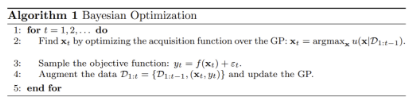
\includegraphics[width=0.75\linewidth]{images/BO.png}
    %\includesvg[width=0.5\linewidth]{images/visual_slam_steps.svg}
	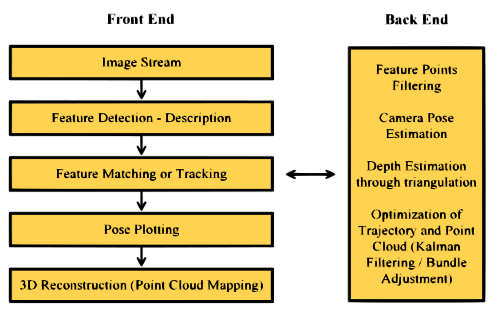
\includegraphics[width=0.75\linewidth]{images/visual_slam_steps.pdf}    
    \caption[Common steps of a generic Visual SLAM system.]{Common steps of a generic Visual SLAM system~\cite{tareen2019large}.}
    \label{fig:enter-label}
\end{figure}

\paragraph{}Firstly, sensor data is collected from the different onboard sensors, such as cameras, \ac{LiDAR}s, \ac{IMU}'s, etc. Given that most systems have sensors that collect data at different frequencies, it is critical for the data to be time-aligned. All data is timestamped relative to a common clock (system clock). This synchronization step ensures that features, poses and inertial readings from multiple sensors correspond to the same physical moment~\cite{macario2022comprehensive}.

%sensors the system has

\paragraph{}Next, features are detected. In the case of Visual \ac{SLAM}, this tipically mean detecting corners, which are often present in more than one frame, allowing for later matching of the same 3D points and for the estimation of the pose of the robotic system. Popular choices for corner detectors are the Harris detector~\cite{harris1988combined} and the blob detector~\cite{lindeberg1998feature, lowe2004distinctive}.%Popular choices for corner detectors are the Harris detectors, which detects points with large intensity changes across two perpendicular directions~\cite{harris1988combined}, and blob detectors(gaussian or laplacian based), which detect regions where the \ac{LoG} or \ac{DoG} response is extreme in scale and space~\cite{lindeberg1998feature, lowe2004distinctive}.

\paragraph{}Feature matching is simply the process of searching for pairs of feature descriptors across different image frames that likely correspond to the same 3D scene point~\cite{liao2024local}. %The simplest and most common baseline matching algorithms simply compare every descriptor in image A with every descriptor in image B and compute a distance metric (euclidean, hamming, etc), which "describes" the similarity between two descriptors. The smaller the distance, the more similar the descriptors are, and therefore, the chance the descriptors correspond to the same 3D point is higher as well~\cite{image_feature_matching}.

\paragraph{}Pose plotting is the process of estimating and visualizing the pose of a moving camera or robot system within a global coordinate frame over time. Each pose represents a snapshot of where the sensor was located and how it was oriented when an image or measurement was captured. By connecting these poses, one obtains a trajectory that shows the motion path through the environment. Accurate pose plots are essential for evaluating localization performance, identifying drift, and debugging SLAM algorithms. Pose plotting relies on solving geometric constraints between observed image features across frames, often using techniques such as Perspective-n-Point (PnP), bundle adjustment, or pose-graph optimization~\cite{chen2018submap}.

\paragraph{}Lastly, 3D reconstruction focuses on building a geometric model of the environment using the estimated poses and visual data. Once camera poses are known, corresponding image features can be triangulated into 3D points to form a map, initially a sparse point cloud and, with additional processing, a dense point cloud~\cite{picard2023surveyrealtime3dscene}. This reconstructed structure represents the physical world captured by the \ac{SLAM} system. High quality 3D reconstruction depends directly on reliable pose estimates, i.e., errors in trajectory estimation propagate into geometric distortions in the map~\cite{picard2023surveyrealtime3dscene, li20213dpointcloudreconstruction}.

\subsection{Types of SLAM solutions}
\paragraph{}If one were to categorize SLAM solutions using the sensor types as a criteria, three broad categories would emerge: Visual \ac{SLAM}(VSLAM), \ac{LiDAR} \ac{SLAM} and multi sensor \ac{SLAM}.

\subsubsection{Visual SLAM}
\paragraph{}Visual \ac{SLAM} uses cameras to understand an environment by detecting and tracking features over time~\cite{chen2018review}. Common subtypes of Visual \ac{SLAM} are (according to the type of camera they use): Monocular SLAM, which uses only one camera, Stereo \ac{SLAM}, which uses 2 cameras, separated by a known baseline, and RGB-D SLAM, which uses cameras that in addition to visual and color information, also provide pixel depth data (distance from camera to an object).

\begin{figure}[h]
    \centering
    \includegraphics[width=0.75\linewidth]{images/VSLAM.png}
    \caption[Visual SLAM feature detection and tracking (left) and 3D reconstruction (right).]{Visual SLAM feature detection and tracking (left) and 3D reconstruction (right)~\cite{danicasado2021}.}
    \label{vslam-example}
\end{figure}

\paragraph{}In terms of hyperparameters, let us consider a few of the most important ones and their effect on the performance of the visual \ac{SLAM} system. When performing feature detection and matching (Figure \ref{vslam-example}), a few important parameters are: \textbf{feature matching threshold}, \textbf{feature detection sensitivity} and the \textbf{scale factor} (in the case of pyramid-based detectors). The \textbf{feature matching threshold} determines how similar two feature descriptors must be to be considered a valid correspondence~\cite{fontan2024anyfeature}. It directly affects how the system associates points between frames or keyframes. A high threshold ensures that only highly similar descriptors are matched~\cite{fontan2024anyfeature}, which increases precision but risks losing correspondences when illumination or viewpoint changes. A low threshold increases the number of matches but allows more outliers, which can corrupt motion estimation~\cite{fontan2024anyfeature}. The \textbf{feature detection sensitivity} defines how easily the detector identifies keypoints in an image, usually based on a response strength or cornerness threshold. A higher sensitivity results in many detected features, improving robustness in textured environments, but it adds computational cost and potential noise. A lower sensitivity limits detections to the strongest points, making tracking faster but potentially unstable in low-texture areas. Lastly, the \textbf{scale factor} (only applicable for pyramid-based detectors) determine how much each image pyramid level is downsampled relative to the previous level~\cite{lindeberg1998feature}. A smaller scale factor adds more levels, improving the ability of the system to handle zooming and depth, but at the cost of aditional computational cost~\cite{lindeberg1998feature}. A higher  scale factor reduces the robustness to scale variations but speeds up feature extraction~\cite{lindeberg1998feature}. In short, this parameter controls a trade-off between real time performance and scale invariant tracking.

\paragraph{}On the topic of pose estimation, \ac{RANSAC} is a particularly important algorithm, which iteratively fits a model to random subsets of data to find the best model that ignores outliers. Specifically, the \textbf{maximum number of iterations} and the \textbf{minimum number of data points} to fit the model are important parameters. The \textbf{maximum number of iterations} specifies how many hypotheses \ac{RANSAC} should run when estimating the camera pose. A higher value increases the probability of finding a correct model, even with many outliers, but adds computational cost~\cite{raguram2008comparative}, while a lower value is too permissive when accepting points into the model, and  can lead to unreliable pose estimates~\cite{raguram2008comparative}. This is a trade-off between robustness to outliers and real time performance. The \textbf{minimum number of data points} (or minimum inlier count) controls how many features correpondences are required to accept a pose estimation as valid. A low value makes the system acccept unstable or incorrect poses, resulting in drift, while a high value might make tracking unfeasible, when very few feature matches are available~\cite{raguram2008comparative}.

\paragraph{}Finally, on the topic of loop closure, the \textbf{loop detection threshold} is one of the most important parameters, which determines how similar two keyframes must be (using a bag of words similarity score, for instance)~\cite{yan2019illumination}. A high threshold only triggers loop closure on highly confident matches. This prevents some false positives but might miss some oportunities to correct drift~\cite{yan2019illumination}. A low threshold increases loop closure sensitivity, but can incorrectly detect loops that might corrupt the map~\cite{yan2019illumination}.


\paragraph{}It should be noted that these parameters are only a fraction of the total number of parameters at play in visual \ac{SLAM} solutions, and are only briefly mentioned here. Also, other, more \textit{exotic}, less used methods might be used throughout the execution of the VSLAM algorithm, which requires a different set of hyperparameters that those presented previously.

\subsubsection{\ac{LiDAR} \ac{SLAM}}
\paragraph{}\ac{LiDAR} \ac{SLAM} uses, as the name suggests, \ac{LiDAR} sensors, which unlike Visual \ac{SLAM}, can measure distances directly using laser pulses. It is overall a more robust method for low light and featureless environments~\cite{lidar_sota}.

\begin{figure}[h]
	\centering
	%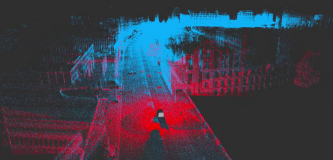
\includegraphics[width=0.75\linewidth]{images/lidar_point_cloud.svg}
	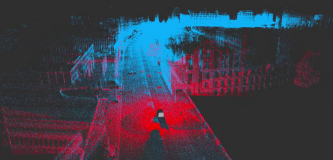
\includegraphics[width=0.75\linewidth]{images/lidar_point_cloud.pdf}
    \caption[LiDAR SLAM point cloud example.]{LiDAR SLAM point cloud example~\cite{slam_point_cloud}.}
    \label{lidar-point-cloud-example}
\end{figure}

\paragraph{}In terms of hyperparameters, a few of the most important hyperparameters often present in \ac{LiDAR} based \ac{SLAM} methods are: \textbf{voxel size}, \textbf{map resolution}, \textbf{maximum correspondence distance} and \textbf{keyframe insertion threshold}. The \textbf{voxel size} determines how much the \ac{LiDAR} point cloud (Figure \ref{lidar-point-cloud-example}) is downsampled before registration. A smaller value helps to preserve detail and accuracy, but sharply increases computation time and noise sensitivity~\cite{zhu2025research}. Larger voxels speed up the system and are more robust to noise, but might increase drift in the process~\cite{zhu2025research}. The \textbf{map resolution} affects the granularity of the internal representation (voxel grid). A high resolution captures more fine-grained features but consumes more memory and processing time~\cite{jorge2024impact}, while a coarse map runs faster but loses detail, affecting localization accuracy~\cite{jorge2024impact}. The \textbf{maximum correspondence distance} determines how far two points can be from each other to be considered a match during scan registration. If too small, the algorithm (\ac{ICP}, \ac{NDT}) may fail to produce enough correspondences, leading to unstable pose estimations~\cite{wang2023comparative}. On the other extreme, if the value set is too high, then incorrect matches will introduce more drift and distort the produced map~\cite{wang2023comparative}. The \textbf{keyframe insertion threshold} (based on distance, for example) controls how often new keyframes are created. Low thresholds yield many keyframes, increasing accuracy but slowing optimization, while high thresholds risk under sampling, introducing drift and lowering loop closure detection~\cite{stathoulopoulos2024sample}.

\subsubsection{Multi-Sensor SLAM}

\paragraph{}Multi-Sensor SLAM encompasses \ac{SLAM} solutions which make use of different types of sensors, taking advantage of the strengths of each one, making the final map and trajectories more robust than if each sensor was used on an independent \ac{SLAM} system.

%is simply a category for the

\begin{figure}[h]
    \centering
    %\includegraphics[width=0.75\linewidth]{images/lidar_SLAM.jpg}
    \includesvg[width=0.75\linewidth]{images/multisensor_slam.svg}
    \caption[Multi-Sensor SLAM system for an industrial robot.]{Multi-Sensor SLAM system for an industrial robot~\cite{multi_sensor_slam_arm_robot}.}
    \label{industrial-robot-slam}
\end{figure}

\paragraph{}A few common multi sensor \ac{SLAM} solutions include: visual inertial \ac{SLAM}~\cite{visual_inertial} (Figure \ref{industrial-robot-slam}), LiDAR inertial \ac{SLAM}~\cite{liu2024voxelslamcompleteaccurateversatile} and visual-lidar-inertial \ac{SLAM} ~\cite{liu2023lidarinertialvisualslamloopdetection}. \textbf{Visual inertial \ac{SLAM}} combines the spatial information from a camera with the higher temporal resolution of an \ac{IMU} to make up for the other sensor's weaknesses. When the \ac{IMU} accumulates too much drift, the cameras help correct it, and the \ac{IMU} helps under poor visual conditions. Its main disadvantage is the high sensitivity to visual degradation, such as fog and dark areas. \textbf{LiDAR-Inertial \ac{SLAM}}'s main advantage is the high robustness in low light or outdoor environments and the resilience to visual noise, present in nightly, foggy and even dusty environments. Two main limitations are the more expensive/heavier setups and the limitation in texture representation (pure geometry only). In \textbf{Visual-Lidar-Inertial \ac{SLAM}}, rich visual features, accurate range data and motion tracking are all present. It however requires a complex calibration and synchronization process, being more expensive and requiring more computational power than simpler multi sensor approaches to \ac{SLAM}.

%\paragraph{}In terms of hyperparameters, multi sensor \ac{SLAM}'s paramaters are largely an amalgamation of their individual sensor constituents.

\subsection{Evaluation of SLAM}
\paragraph{}Assessing \ac{SLAM} performance requires quantitative and qualitative metrics that evaluate how accurate, robust and efficient the estimated map and trajectory are. A few evaluation criteria include the \ac{ATE}, Relative Pose Error (RPE), resource usage (memory and CPU time consumption), etc.

\paragraph{}The \textbf{\ac{ATE}} measures the global deviation between estimated and ground truth trajectories. At each point in the trajectory, the difference between the estimated pose and the ground truth pose is computed. For a more general measure of the \ac{ATE}, one might also calculate the \ac{RMSE}, as follows:

\begin{center} 
    \begin{equation} 
        ATE_{RMSE} = \sqrt{\frac{1}{N}\sum_{i=1}^{N}\|S(p_i^{est}) - p_i^{gt}\|^2}.
    \end{equation}
\end{center}

\paragraph{} The \textbf{\ac{RPE}} measures the local consistency of the trajectory by evaluating the difference in relative motion between estimated and ground truth poses over a fixed time interval. As with the \ac{ATE}, the formula for the \ac{RMSE} of the \ac{RPE} is as follows:

\begin{center}
    \begin{equation}
        RPE_{RMSE} = \sqrt{\frac{1}{N}\sum_{i=1}^{N}\|(T_i^{est})^{-1}T_{i+\Delta t}^{est} - (T_{i}^{gt})^{-1}T_{i+\Delta t}^{gt}\|^2}.
    \end{equation}
\end{center}

\paragraph{}It is important to take into account the system resource utilization, both the memory and CPU time consumption, when benchmarking and comparing different \ac{SLAM} solutions, due to the trade-offs between accuracy/noise robustness and memory utilization/time consumption. %Depending on the application, it might not be worth it to use a more computationally intensive (but more accurate) \ac{SLAM} solution.

\paragraph{}In addition to the metrics mentioned previously, one might want to optimize for other metrics not included on this list. In that case, it might be useful to use a fitness function where normalized weights are attributed to each metric, according to the importance of each metric. %has to the user.

\paragraph{}Finally, when evaluating and comparing different \ac{SLAM} solutions, it is important to establish a fair playing field for all the algorithms to be compared. One of the ways to do that is to use publicly available standardized datasets, such as the KITTI Dataset~\cite{kitti_dataset}. As for evaluation frameworks, one of the most widely used is EVO~\cite{grupp2017evo}, which provides error metrics and visualization tools, so as to better compare the performance of different \ac{SLAM} solutions.

\section{Parameter optimization techniques}
\paragraph{}Parameter optimization techniques can be broadly categorized into search-based, model-based and population-based approaches. Each approach uses different strategies to search the parameter space and obtain an approximation of the optimal solution, such as randomly sampling configurations (random search), mimicking physical processes to get a faster convergence (Simulated Annealing) or even by pre-selecting a parameter space and dropping half of the worst performing configurations at each pass (successive halving). Some of these approaches require a budget to be defined, meaning a time limit, or a maximum number of configurations to be tested.

\subsection{Search based approaches}

\paragraph{}One popular type of approach to the problem of \ac{HPO}, which will be used as a baseline on this dissertation's work, is a search based approach, such as Grid Search and Random Search. These approaches are popular due to their implementation simplicity and paralelization possibilities.

\subsubsection{Grid Search}

\paragraph{}Grid Search is a basic solution for \ac{HPO}. It simply consists of an exhaustive search and evaluation of all possible hyperparameter combinations within a predefined parameter space~\cite{yang2020hyperparameter} (Figure \ref{grid-search-plot}). In spite of the development of more sophisticated and specific algorithms in recent decades, Grid Search remains popular due to its simple implementation and trivial paralelization~\cite{yang2020hyperparameter}. The main drawback is its computational cost, due to the curse of dimensionality being a serious problem in models with large numbers of hyperparameters~\cite{yang2020hyperparameter}. This might be summarized by the following equation:

\begin{equation}
    N_c = \prod_{n=1}^{k} {N_{P_i}},
    \label{equation_grid_search}
\end{equation}

\noindent where $N_c$ is the total number of configurations and $N_{P_i}$ is the number of possible values for hyperparameter i of the model.

Inspection of Equation \ref{equation_grid_search} reveals that this algorithm does not scale efficiently, due to the rapid increase in the number of configurations, which makes this the main hurdle in search based approaches. One way to overcome this is by paralelizing the execution of various configurations across several CPU cores and threads. Another way is to pre-select the parameters to optimize, and/or discarding hyperparameters which have little effect on the model's performance. However, this strategy has its downsides. If the initial analysis of the relevant parameters is inaccurate, parameters that are significant in certain regions of the parameter space may be prematurely discarded~\cite{bergstra2012random}. Additionally, parameters that individually have small effects on the output metric may have greater effects when combined~\cite{bischl2021hyperparameter}.

%By looking at equation \ref{equation_grid_search}, it becomes clear this algorithm is not very scalable

\begin{figure}[h]
    \centering
    \includegraphics[page=1, width=0.6\linewidth]{images/search_tese.pdf}
    \caption[Graphical illustration of parameter space exploration in grid search.]{Graphical illustration of parameter space exploration in grid search~\cite{castillo2022hyperparameter}.}
    \label{grid-search-plot}
\end{figure}

\newpage
\subsubsection{Random Search}

\paragraph{}Random Search is a variation of Grid Search. It randomly samples configurations in the aforementioned parameter space~\cite{bissuel2020hyper} (Figure \ref{random-search-plot}). Both Grid Search and Random Search are very similar implementation wise, with one major difference: Random Search requires a budget to be specified, whether it is time, number of configurations, etc~\cite{bergstra2012random}. Compared to Grid Search, Random Search offers faster convergence toward local or global optima~\cite{bergstra2012random}; however, this advantage becomes less pronounced as the parameter space grows.

%The main advantage Random Search has over Grid Search is the faster convergence over a local or global optima~\cite{bergstra2012random}, although this advantage gets slimmer the larger the parameter space.

\begin{figure}[h]
    \centering
    \includegraphics[page=2, width=0.5\linewidth]{images/search_tese.pdf}
    \caption[Graphical illustration of parameter space exploration in random search.]{Graphical illustration of parameter space exploration in random search~\cite{castillo2022hyperparameter}.}
    \label{random-search-plot}
\end{figure}

\newpage
\subsection{Model based approaches}

\paragraph{}Model based approaches tackle the optimization problem in a different way, by building a surrogate model that describes the relationship between hyperparameter configurations and algorithm performance. The inner workings of the algorithm to be optimized are unspecified and it is therefore treated as a black box~\cite{morales2023survey}. These kind of HPO techniques are better suited to more complex optimization problems and clarify the relationship between algorithm performance and hyperparameter settings, which might prove to be an appropriate option to pre-select the most important hyperparameters to optimize when there are dozens or hundreds of parameters.

\subsubsection{Bayesian Optimization}

\paragraph{}\ac{BO} is a probabilistic model-based approach that optimizes black box functions that are expensive to evaluate~\cite{mockus1998application}. It is particularly useful when the objetive function lacks an analytic expression and its evaluation is expensive, which is the case for \ac{SLAM} methods.

\begin{figure}[h]
\centering
\begin{algorithm}[H]
\caption{Bayesian Optimization}
\begin{algorithmic}[1]
\For{$t = 1, 2, \ldots$}
    \State Find $x_t$ by optimizing the acquisition function over the Gaussian Process (GP):
        \[
            x_t = \arg\max_x \, u(x \mid \mathcal{D}_{1:t-1})
        \]
    \State Sample the objective function: $y_t = f(x_t) + \epsilon_t$
    \State Augment the data $\mathcal{D}_{1:t} = \{\mathcal{D}_{1:t-1}, (x_t, y_t)\}$ and update the GP.
\EndFor
\end{algorithmic}
\end{algorithm}
\caption[Bayesian Optimization algorithm steps.]{Bayesian Optimization algorithm steps~\cite{brochu2010tutorial}.}
\label{bo_algo}
\end{figure}

\paragraph{}Bayesian Optimization has two main components:
\begin{itemize}

    \item A Surrogate model, which is a probabilistic, fast proximate model that stands in for, and is much easier to evaluate than, an unknown (black box) or expensive function~\cite{elshawi2019automated}. Instead of repeatedly evaluating the true function, which might take a long time, the surrogate model (usually a Gaussian Process~\cite{bissuel2020hyper}) learns from previous evaluations, and predicts both the expected mean value of the true function (in this case, the \ac{RMSE} of the \ac{RPE} of a \ac{SLAM} solution) and the uncertainty at each point. The uncertainty is what informs and guides the algorithm on what point to sample next, by balancing promising regions with unexplored ones (higher uncertainty).
    
	\item An Acquisition function, which is the rule \ac{BO} uses to choose the next objective function point to evaluate~\cite{elshawi2019automated}. It uses the surrogate model's predictions (mean and uncertainty) and combines them into a single score, which is then used to evaluate the best candidate point. Common Acquisition functions include \ac{PI}, which focuses on the \textbf{chance} of beating the current best result, and \ac{ULCB}, which explicitly trades-off mean and uncertainty using a tunable hyperparameter~\cite{frazier2018tutorial}.
	
\end{itemize}

\paragraph{}\ac{BO} uses the following iterative process to optimize the objetive function (see Figure \ref{bo_algo}):
\begin{enumerate}
    \item Select the next point to be sampled with the aquisition function.
    \item Evaluate the true function $f(x_1, x_2 ... x_n)$ at the selected point.
    \item Update the surrogate model with the new information using gaussian process regression, which is the process of adding additional information of the sampled points to the \textbf{prior}.
    \item Repeat steps 1, 2 and 3 until some stopping criteria is met (exhausted budget, achieved convergence, etc).
\end{enumerate}

\paragraph{}One major drawback of Bayesian Optimization is the impossibility of paralelization when compared to other baseline techniques, due to the fact the the surrogate model uses new points to update its parameters, meaning the learning process needs to finish before a new one can be launched~\cite{bissuel2020hyper}.

\subsection{Population based Approaches}
\paragraph{}These types of approaches are defined by a population of candidate solutions (sets of hyperparameters) that are iteratively updated to optimize an objetive function~\cite{kostusiak2019efficiency}, such as the \ac{APE} or the \ac{RPE} in the case of \ac{SLAM} optimization.

\subsubsection{Simulated Annealing}

\paragraph{}\ac{SA} is a meta-heuristic that mimicks the physical process of heating a metal and then cooling it slowly~\cite{rutenbar1989simulated}. Analogously, the algorithm freely explores solutions in the beginning, even ones that seem worse at face value, so as to maximize exploration, and then, as the temperature decreases, according to a predefined cooling schedule, it focuses on refining a solution~\cite{ghasemalizadeh2016review, rutenbar1989simulated}.

\paragraph{}The method starts by assigning an initial value to each hyperparameter, one that is high enough to allow compreensive search over the parameter space~\cite{ghasemalizadeh2016review}, due to the high variance of the parameter values in early stages of the algorithm. Then, it makes small changes to each parameter at a time and evaluates this new configuration, called a neighbor~\cite{rutenbar1989simulated}. The acceptance of the neighbor as being a superior solution depends on a probabilistic distribution~\cite{rutenbar1989simulated}, which in itself depends on the temperature and the difference between the current solution's and the neighbor solution's evaluation, like so:

\begin{equation}
	P = e^{-\frac{\Delta E}{T}},
\end{equation}

\noindent where T is the current temperature and $\Delta E$ is the difference between the cost of the new solution (the neighbor's) and the cost of the current solution, that is, $\Delta E = f'(x) - f(x)$.

\paragraph{}Then, the algorithm updates the temperature, using the following expression: $T' = \alpha T$, where $\alpha$ is the cooling factor, which is usually given a value in the interval [0.8, 0.99].

\paragraph{}The algorithm repeats the previous steps until the temperatures reaches a minimum value or a stopping condition is triggered, such as a maximum number of iterations \cite{ghasemalizadeh2016review}. Once execution stops, the best solution is returned as an approximation to the actual optimal solution. Figure 2.8 shows a graphic representation of \ac{SA}’s behavior.

\begin{figure}[h]
    \centering
    %\includesvg[width=0.4\linewidth]{images/SA.svg}
    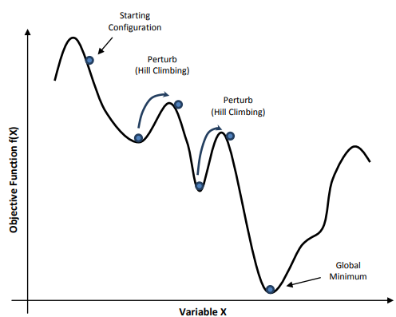
\includegraphics[width=0.5\linewidth]{images/SA.pdf}
    \caption[A graphic representation of the Simulated Annealing algorithm.]{A graphic representation of the Simulated Annealing algorithm~\cite{sa_netlogo}.}
    \label{fig:enter-label}
\end{figure}

\subsubsection{Successive Halving}

\paragraph{}\ac{SH} is an optimization method that efficiently allocates resources to the most promising configurations while reducing investment into less promising ones~\cite{soper2021greed}. Similar to \ac{SA}, this technique requires a budget to be specified (execution time, number of iterations, etc.).

\paragraph{}At first, $n$ candidates are generated and evaluated, and the constrained resources are assigned equally to all configurations. Then, \textbf{the worst half of all configurations is discarded} and this process is repeated until only 1 configuration remains~\cite{huang2019survey}. The hyperparameter configurations used in this method can be generated in a variety of different ways. A popular one is identical to the way parameter spaces are generated in Grid/Random Search algorithms, where the researcher manually selects the parameters to optimize, as well the their upper and lower bounds, as well as the step size.%One can define a parameter space similar to the one used in search-based approaches and use either Grid Search or Random Search to generate the desired number of configurations. There is also the possibility of manually selecting both the hyperparameters to optimize and their values.

\begin{figure}[h]
    \centering
    %\includegraphics[width=0.5\linewidth]{}
    \includesvg[width=0.6\linewidth]{images/SH.svg}
    \caption[A graphic representation of the Successive Halving algorithm.]{A graphic representation of the Successive Halving algorithm~\cite{soper2022hyperparameter}.}
    \label{fig:enter-label}
\end{figure}

\subsubsection{Hyperband}
\paragraph{}Hyperband is a more efficient technique that builds on the Successive Halving algorithm~\cite{elshawi2019automated}. By dynamically allocating computational resources, Hyperband quickly identifies promising configurations and discards ill-performing ones early on, saving both time and computational resources.

\paragraph{}Hyperband works as follows:

\begin{enumerate}

    \item Define a total Budget B and the proportion of configurations to evaluate at each iteration, $\eta$. Also, a maximum budget R for a single iteration is required~\cite{falkner2018bohb}.

    \item Generate a large number of configurations~\cite{falkner2018bohb}.

    \item Allocate a small initial budget to all configurations and perform the successive halving algorithm with one modification: halt its execution when only the top 1 / $\eta$ configurations remain, instead of halting when only the best configuration remains. Then, increase the budget for the remaining configurations~\cite{falkner2018bohb}.

    \item Repeat step 3 until maximum budget R is reached or all configurations are exhausted, meaning only the best one remains~\cite{falkner2018bohb}.

\end{enumerate}

By increasing the budget allocated to a decreasing number of configurations at each execution of the Successive Halving algorithm, Hyperband transitions from an exploration-focused method to an exploitation-focused one.

\begin{figure}[h]
    \centering
    \includegraphics[width=0.75\linewidth]{images/hyperband.pdf}
    %\includesvg[width=0.65\linewidth]{images/Hyperband.svg}
    \caption[Hyperband described in a more systematic way.]{Hyperband described in a more systematic way~\cite{li2018hyperband}.}
    \label{fig:enter-label}
\end{figure}

\subsection{\acs{HPT} in \acs{SLAM}}

%\paragraph{}When applying \ac{HPT} algorithms to fine tune a \ac{SLAM} method's parameters, there are a few things to keep in mind.

%\paragraph{}First, not all parameters are tunable. Better yet, some parameters have fixed or default values and are treated as constants during the tuning process, such as a camera's intrinsic parameters in VSLAM, or an IMU's noise and Bias models in Visual-Inertial \ac{SLAM}. This is an important aspect to keep in mind, especially when applying search based approaches, as it may provide a way to significantly reduce the number of configurations to be executed.

%\paragraph{}As it pertains to the effectiveness of tuning strategies, search based methods are usually considered baseline methods in research, and not very effective when dealing with very high dimensional parameter spaces, due to the high stochasticity of grid and random search. In this regard, simulated annealing achieves better results, incorporating local refinement and controlled exploration. But in order to obtain near optimal results, and faster, other approaches are needed. Successive Halving and Hyperband work well within constrained environments(hardware, time etc), and Bayesian Optimization surpasses the previous 2 strategies in sample efficiency(how many full evaluations of the objective function are necessary to find a good configuration). Bayesian Optimization also works very well when the objective function is expensive to evaluate, or when the parameter space is low dimensional, which might be the case in a \ac{SLAM} setting, provided the researcher carefully hand-picks the parameters to optimize.

\paragraph{}When optimizing the parameters of a \ac{SLAM} method, several considerations must be taken into account.

\paragraph{}First, not all parameters are amenable to tuning. In practice, some parameters have fixed or default values and are treated as constants throughout the tuning process, such as camera intrinsic parameters in visual \ac{SLAM}, or the noise and bias models of an \ac{IMU} in Visual–Inertial \ac{SLAM}. This distinction is particularly important when employing search-based approaches, as excluding non-tunable parameters can substantially reduce the size of the search space and, consequently, the number of configurations that must be evaluated.

\paragraph{}With respect to the effectiveness of different tuning strategies, search-based methods are typically regarded as baseline approaches in the literature and tend to perform poorly in high-dimensional parameter spaces due to the inherent stochasticity of Grid and Random Search. In contrast, Simulated Annealing generally yields improved results by incorporating both local refinement and controlled exploration of the search space. However, achieving near-optimal solutions in a computationally efficient manner often requires more advanced techniques. Methods such as Successive Halving and Hyperband are well suited to constrained environments, where computational resources or time are limited. Bayesian Optimization further improves upon these approaches in terms of sample efficiency, as it typically requires fewer full evaluations of the objective function to identify high-performing configurations. Moreover, Bayesian Optimization is particularly effective when objective function evaluations are expensive or when the parameter space is low dimensional, which may be the case in some \ac{SLAM} contexts, provided that the parameters to be optimized are carefully selected by the researcher.

\section{Related Work}

\paragraph{}This subsection discusses published research in optimizing parameters in \ac{SLAM} systems. It presents a brief description of each relevant article and the used \ac{SLAM} method and optimizing strategy, as well as the results from the experiments that were made. It then goes over the current literature research gaps and presents the main contributions of this dissertation.

\paragraph{}On search-based approaches, there has been some research on the topic. Particularly, Putra et al. have hand-selected and manually searched (brute force) the parameter space of a G-Mapping SLAM solution~\cite{putra2019parameter}. In this specific case, four parameters were tuned: \textbf{linear update step}, \textbf{angular update step}, \textbf{quantity of particle}, and \textbf{resampling threshold}. The particle number directly determines the number of possible robot position hypotheses the algorithm tracks. The linear update step is the minimum distance (in meters) the robot must move before updating the map. Similarly, the angular update step is the minimum angle the robot must rotate before triggering a map update. Finally, the resampling threshold controls the frequency at which particles are resampled. Through several executions of the algorithm, it was possible to reduce the navigation time of a robot from 32 seconds to 25 seconds.

\paragraph{}Another study applied grid search to optimize 5 parameters in a feature based monocular visual odometry setting~\cite{zheng2020feature}. In all 10 sequences, measured ATE significantly decreased, showing the main advantage of this simple tuning approach. Naturally, the optimal configuration wasn't the same in all sequences, showing that a parameter's optimal value depends on the dataset for which it is optimized, in order to find a balanced setup, the authors chose parameter values that consistently produced reduced \ac{ATE} values across all sequences. It is also worth noting that while search based approaches are more suited for a parameter set, Grid Search is generally preferable to manual (Brute-force) search. Additionally, both previously discussed articles indicate that, given knowledge of the system, the parameter space may be reduced to a limited set of influential parameters, allowing Grid and Random Search to yield configurations that improve upon default settings.

%Additionally, both papers presented previously show that, with good knowledge of the system, one can significantly reduce the parameter space down to the very few and impactful hyperparameters and achieve a significantly better configuration than a default one when using grid and random search.

\paragraph{}As far as model based approaches go, \ac{BO} is the most used algorithm in research. One paper used a variant of it, \ac{SMBO} to optimize the hyperparameters of a LiDAR-based Odometry algorithm, without knowledge of the  inner workings of the system, e.g the system is treated as a black box~\cite{koide2021automatic}. Although data augmentation was used to prevent overfitting (by adding random noise to the point clouds, reversing the data order, and applying a random transformation to the point cloud), it was still possible to observe a noticeable decrease in the odometry drift error (in most tested sequences). Although beyond the scope of this dissertation (in which camera parameters are treated as constants), another work applied Bayesian Optimization to optimize the extrinsic parameters of a camera in a Visual-Inertial \ac{SLAM} system~\cite{chen2018visual}.

%Another article, although outside the scope of this dissertation(in this dissertation, camera parameters are considered constants) used \ac{BO} to fine tune the extrinsic parameters of a camera in a Visual Inertial \ac{SLAM} system~\cite{chen2018visual}.

\paragraph{}With regards to population-based approaches, relatively little research has been conducted specifically in the context of \ac{SLAM}. However, a study by Kostusiak and Skrzypczyński~\cite{kostusiak2019efficiency} used a \ac{PSO} algorithm and an \ac{EA} to tune the parameters of an RGB-D Visual Odometry system to improve motion estimation accuracy. Using the TUM RGB-D dataset for training and the PUT Kinect dataset for testing, the authors applied the two previously mentioned methods to adjust only five influential hyperparameters related to feature detection (AKAZE feature detector threshold) and outlier rejection (two \ac{RANSAC} distance and inlier/outlier thresholds)~\cite{kostusiak2019efficiency}. The optimization, guided by the values of the \ac{ATE} and \ac{RPE}, showed that tuning these few parameters, particularly the AKAZE feature threshold and \ac{RANSAC} distance limits, significantly reduced trajectory errors, with ATE dropping from about 1.6m to 0.29m~\cite{kostusiak2019efficiency}. While the Particle Swarm algorithm achieved the best accuracy out of the 2 tuning strategies, the Evolutionary Algorithm achieved similar results in one-fifth of the time~\cite{kostusiak2019efficiency}. Alternatively, the authors also manually tuned the parameters, with significantly inferior results than \ac{PSO}~\cite{kostusiak2019efficiency}.

\begin{landscape}

\begin{table}
\centering
\footnotesize
  \begin{tabular}{@{} p{0.25\textwidth} p{0.3\textwidth} p{0.3\textwidth} p{0.3\textwidth} @{}}
    \toprule
	Article(s) &  SLAM category  & Optimization method(s) & Results \\
    \addlinespace
    \hline
    
	Z. Zheng (2020)~\cite{zheng2020feature} & Feature-based Visual Odometry (not full \ac{SLAM}) & Grid Search & Across 8 optimized sequences, average ATE decreased, on average, 64.68\%\\
    \addlinespace
    
	A. Putra and P. Prajitno (2019)~\cite{putra2019parameter} & G-mapping SLAM (particle filter) & Brute Force & Navigation time of a predefined path was reduced from 32 to 25 seconds \\
    \addlinespace   
    
	K. Koide et al (2021)~\cite{koide2021automatic} & Lidar Odometry (not full \ac{SLAM}) & based on Bayesian Optimization &  \textbf{With data augmentation}, in both tested environments, drift error decreased by at least 9.8\% \\
	\addlinespace 
	
	A. Kostusiak and P. Skrzypczyński (2019)~\cite{kostusiak2019efficiency} & RGB-D Visual Odometry & Particle Swarm Optimization (PSO) & RPE decreased by well over 50\% \\
	\addlinespace
	
	\rule[-0.4ex]{4cm}{1.5pt} & \rule[-0.4ex]{4cm}{1.5pt} & Evolutionary Algorithm (EA) & Similar performance to PSO, but tuning duration is 5x shorter \\
	
	%\multirow{2}{0.3\textwidth}{Particle Swarm Optimization (PSO) \newline Evolutionary Algorithm (EA)} & \multirow{2}{0.3\textwidth}{RPE decreased by well over 50\% \newline Similar performance to PSO, but tuning duration is 5x shorter}\\
	
	\\
    
    \end{tabular}
\caption{Summary of \ac{HPT} methods used in the literature.}
\end{table}

\end{landscape}

\newpage

\subsection{Literature Gaps}
\paragraph{}A few notable research gaps exist in the field of SLAM parameter tuning. Most notably:

\begin{itemize}
    \item Lack of diversity in optimization strategies. As presented earlier, most of the research use either a search-based approach or a model-based approach (similar to \ac{BO}), as well as only using one optimization method for their particular \ac{SLAM} solution. When there is a comprehensive understanding of sensor behavior and the influence of parameters on \ac{SLAM} performance, some parameters may be retained at their default values, allowing a straightforward search-based strategy to optimize the remaining parameters. As for the model-based approaches, they are used most when there is no extensive knowledge of the system at hand. Therefore, \ac{BO} treats it as a black box and optimizes it. Apart from~\cite{kostusiak2019efficiency}, research on population-based approaches for \ac{SLAM} optimization remains scarce, whether variations of particle swarm algorithms, evolutionary algorithms, or other meta heuristics.
    
%For \ac{SLAM} systems where there is a high degree of knowledge of the inner working of the sensors and how different parameters affect the performance of the solution, it is possible to manually set and stick with default values for some of the hyperparameters, and can then apply a simple baseline(search-based) approach to the tuning of the remaining hyperparameters. As for the latter, it is used most when there is no extensive knowledge of the system at hand. Therefore, \ac{BO} treats it as a black box and optimizes it. Apart from~\cite{kostusiak2019efficiency}, there isn't much research on population-based approaches to optimizing \ac{SLAM}, whether variations of particle swarm algorithms, evolutionary algorithms, or other meta heuristics.
    
    \item Lack of frameworks to automatically optimize \ac{SLAM} methods, allowing for an even playing field in \ac{SLAM} research. Athough a framework like \textbf{SLAMBench2}~\cite{bodin2018slambench2multiobjectiveheadtoheadbenchmarking} provides a platform with a controlled dataset and with standardized metrics, it lacks an automatic tuning feature. Similarly, \textbf{\ac{RUSTLE}}\footnote{\url{https://github.com/Forestry-Robotics-UC/rustle}}, the tool which will be built and improved upon during the course of this dissertation, already allows for a somewhat organized approach to testing and optimizing complete \ac{SLAM} solutions, but it lacks any optimization feature, meaning the only way to currently approach \ac{HPT} in RUSTLE is by brute force optimizing an algorithm.
    
\end{itemize}

\subsection{Statement of Contributions}

\begin{itemize}

	\item Implementation of several algorithms for tuning a \ac{SLAM} system's parameters, namely Grid Search, Random Search, and Simulated Annealing
	
	\item Integration of the implemented tuning algorithms into the existing open source framework (\ac{RUSTLE}) to allow for automated and streamlined tuning
	
	\item Validation and testing of the implemented tuning algorithms on two SLAM solutions

\end{itemize}

%\paragraph{}Given that academic research often focuses on a single optimization method for a particular \ac{SLAM} system for an even more specific use case, the main contribution of this dissertation is new software features(within \ac{RUSTLE}) for the optimization of multiple \ac{SLAM} solutions in an organized and systematic manner.